\documentclass[convert = false, tikz]{standalone}
\usepackage[utf8]{inputenc}
\usepackage{tikz}
\usetikzlibrary{automata, positioning, arrows, shapes.geometric, decorations.pathmorphing}

\usepackage{../../../../style_automata}

% arara: pdflatex
% arara: latexmk: { clean: partial }
\begin{document}
    \tikzset{
    node distance=2cm, % specifies the minimum distance between two nodes.
    }
    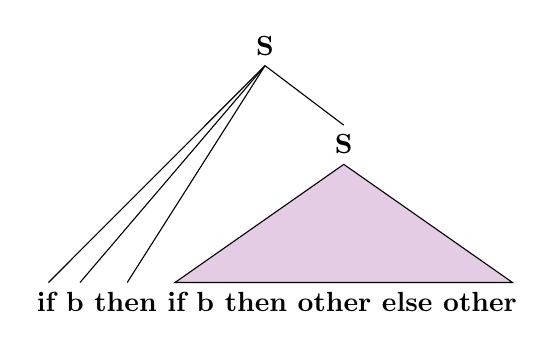
\begin{tikzpicture}

    % Apex angle 60 degrees
    \node[](S1){\textbf{S}};

    \draw[] ([yshift=-1cm, xshift=1cm]S1.south) node[] (S2) {\textbf{S}};

    \draw[] (S2.south) node[isosceles triangle, rotate=90, isosceles triangle apex angle=110, draw, minimum size=1.5cm, anchor=apex, fill=violet!20] (T) {};
    
    \draw[] ([yshift=-3cm, xshift=0.15cm]S1.south) node[] (text) {\textbf{if b then if b then other else other}};
    
    \draw [] (S1.south) -- (S2.north);
    \draw [] (S1.south) -- ([xshift=-1.9cm]text.north);
    \draw [] (S1.south) -- ([xshift=-2.5cm]text.north);
    \draw [] (S1.south) -- ([xshift=-2.9cm]text.north);

    
    \end{tikzpicture}
\end{document}